\documentclass[conference]{IEEEtran}
\IEEEoverridecommandlockouts
% The preceding line is only needed to identify funding in the first footnote. If that is unneeded, please comment it out.
\usepackage{cite}
\usepackage{amsmath,amssymb,amsfonts}
\usepackage{algorithmic}
\usepackage{graphicx}
\usepackage{textcomp}
\usepackage{xcolor}
\usepackage{subcaption}

\usepackage{lipsum}% http://ctan.org/pkg/lipsum

\def\BibTeX{{\rm B\kern-.05em{\sc i\kern-.025em b}\kern-.08em
    T\kern-.1667em\lower.7ex\hbox{E}\kern-.125emX}}

\begin{document}

\title{Use Online Dictionary Learning to Get Parts-based Decomposition of Noisy Data}

\author{\IEEEauthorblockN{Daming Lu}
\IEEEauthorblockA{\textit{Baidu Research} \\
Sunnyvale, CA \\
ludaming@baidu.com}
}

\maketitle

\begin{abstract}
Huge amount of data are generated every day. Extracting interpretable features from the data is becoming important. Meanwhile, dimension reduction and low rank approximation are also becoming important as people want to factorize big matrix into smaller ones, which are easier to handle. Sparse coding is such a technique that can factorize matrix into sparse linear combinations of basis elements. We found that through \textit{Online Dictionary Learning}, an efficient sparse coding algorithm, we could decompose large data matrix with noise into interpretable dictionary atoms. Such atoms are useful in reconstructing a denoised data matrix.
\end{abstract}

\begin{IEEEkeywords}
machine learning, sparse coding, online dictionary learning, dimension reduction
\end{IEEEkeywords}

%-%-%-%-%-%-%-%-%-%-%-%-%-%-%-%-%-%-%-%-%-%-%-%-%-%-%-%-%-%-%-%-%-%-%-%
\section{Introduction}
Large amount of high dimensional data are generated every day, thanks to the prosperity of the Internet and big data technology. Due to the difficulty of processing high dimensional data, people intend to factorize or decompose large data matrices into smaller ones. The linear decomposition of a matrix into a few basis elements has been a hot research spot for a long time. At first, general purposed basis matrices were used to represent the large matrix, such as wavelets \cite{b1}. Later, using \textit{ad hoc} matrix learned from specific input data could produce better results. However, although many such decomposition methods could produce smaller matrices, most of these matrices are hardly interpretable, especially when the input data are noisy. Such popular methods include principal component analysis (PCA) \cite{b2}, CUR matrix decomposition \cite{b3}, etc. We found that the \textit{Online Dictionary Learning} method, introduced in \cite{b4}, could not only reduce the matrix dimension, but also get the atoms in the learned dictionary that are interpretable. We applied this technology to two different sets of noisy data and found the extracted atoms very close to the ground truth.

We compared our method with \textit{UoI-NMF\textsubscript{cluster}} \cite{b5} and found our accuracies are better. Meanwhile, we found that \textit{Online Dictionary Learning} runs faster as it does not require the clustering step as in \textit{UoI-NMF\textsubscript{cluster}}. The clustering step is actually crucial for robustness. As a result, \textit{UoI-NMF\textsubscript{cluster}} is more robust compared to \textit{Online Dictionary Learning}, which will be discussed in Section 4. The following sections are organized as below:

\begin{itemize}
\item We first review the core part of \textit{Online Dictionary Learning}.
\item We then introduce the application of \textit{Online Dictionary Learning} on our datasets and compare the results with \textit{UoI-NMF\textsubscript{cluster}}.
\item Finally we discuss potential advantages and disadvantages of both methods.
\end{itemize}

%-%-%-%-%-%-%-%-%-%-%-%-%-%-%-%-%-%-%-%-%-%-%-%-%-%-%-%-%-%-%-%-%-%-%-%
\section{PRELIMINARIES}
\subsection{Online Dictionary Learning}

\textit{Online Dictionary Learning} was first introduced in \cite{b4}. Assume we have a finite training dataset as $ X=[x_1,...x_n] $ in $R^{m\times n}$, we want to learn a dictionary $D$ as a ``good'' representation of signal $x$. Normally the dimension $m$ is relatively small compared to the total amount of data $n$. We want to have a $k\ll n$ such as we can only use a few elements (atoms) in $D$ to represent signal $x$. Our aim is to optimize $\ell(x, D)$ as the $\ell_{1}$ sparse coding problem:
$$ \ell(x, D) \triangleq \min\limits_{\alpha \in R^k} \frac{1}{2}\Arrowvert x-D\alpha \Arrowvert^{2}_{2}+\lambda\Arrowvert \alpha \Arrowvert_{1}$$
where $ \lambda $ is a regularization parameter. This problem is also called \textit{basis pursuit} \cite{b4}, or more commonly, \textit{Lasso}  \cite{b4}. It can be rewritten as a joint optimization problem with respect to the dictionary $D$ and the coefficients $\alpha=[\alpha_1,...,\alpha_n]$ of the
sparse decomposition. Although it is not jointly convex, it can be convex with respect to each of the two variables $D$ and $\alpha$ when
the other one is fixed. An intuitive way of solving this convex optimization problem is to alternatively update one variable with the other one fixed, as proposed in \cite{b4}. Bottou and Bousquet (2008) pointed out that instead of minimizing empirical cost, minimizing expected cost is often more demanding. We chose \textit{Online Dictionary Learning} as it does not require explicit learning
rate tuning and is focused on minimizing a local approximations of the expected cost. We followed the algorithm as mentioned in \cite{b4} with a mini-batch extension in order to prevent polluting the initialization.

%-%-%-%-%-%-%-%-%-%-%-%-%-%-%-%-%-%-%-%-%-%-%-%-%-%-%-%-%-%-%-%-%-%-%-%
\section{NUMERIC EXPERIMENTS}
In this section, we illustrate the application of \textit{Online Dictionary Learning} on two datasets: Swimmer dataset and MNIST 2-digit dataset. The details of these two datasets were introduced in \cite{b5}. We used SPAMS library \cite{b6,b7} as our backbone.

%- plot figures -%

%-MNIST-%
\begin{figure*}[!htb]
\centering
\minipage{0.25\textwidth}
  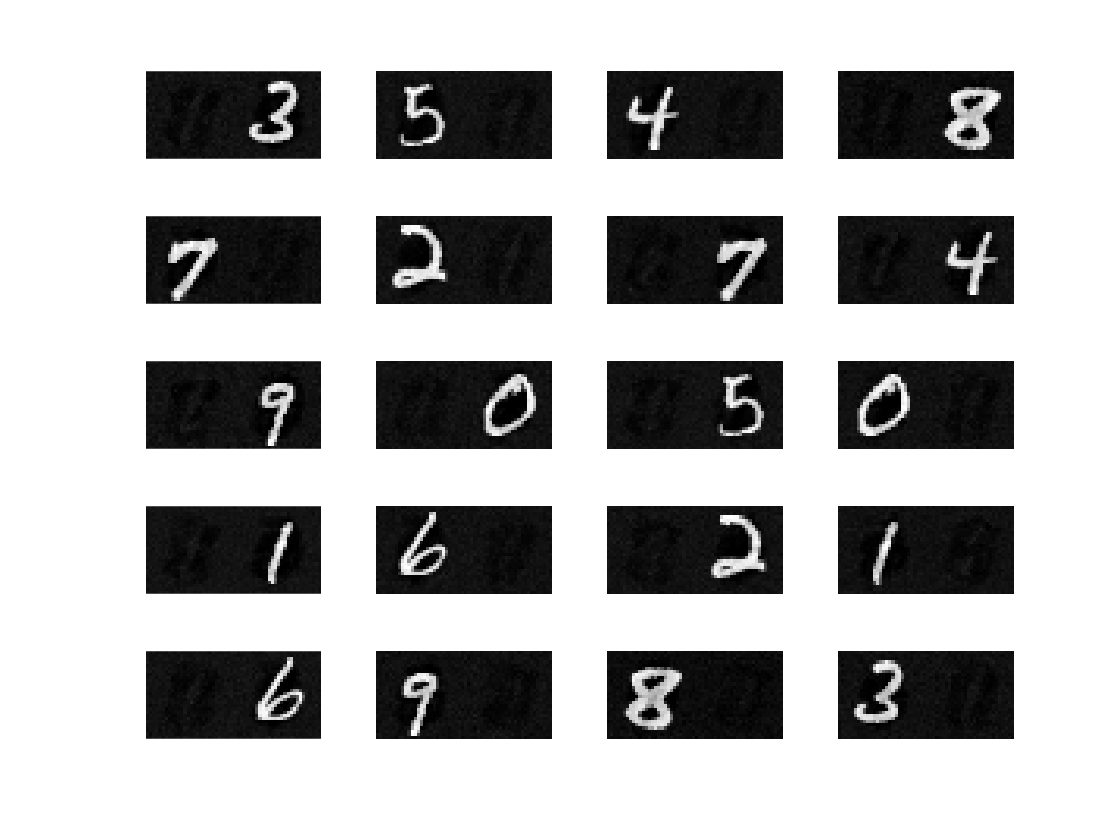
\includegraphics[width=\linewidth]{uoi_best_basis}
\endminipage\hfill
\minipage{0.25\textwidth}
  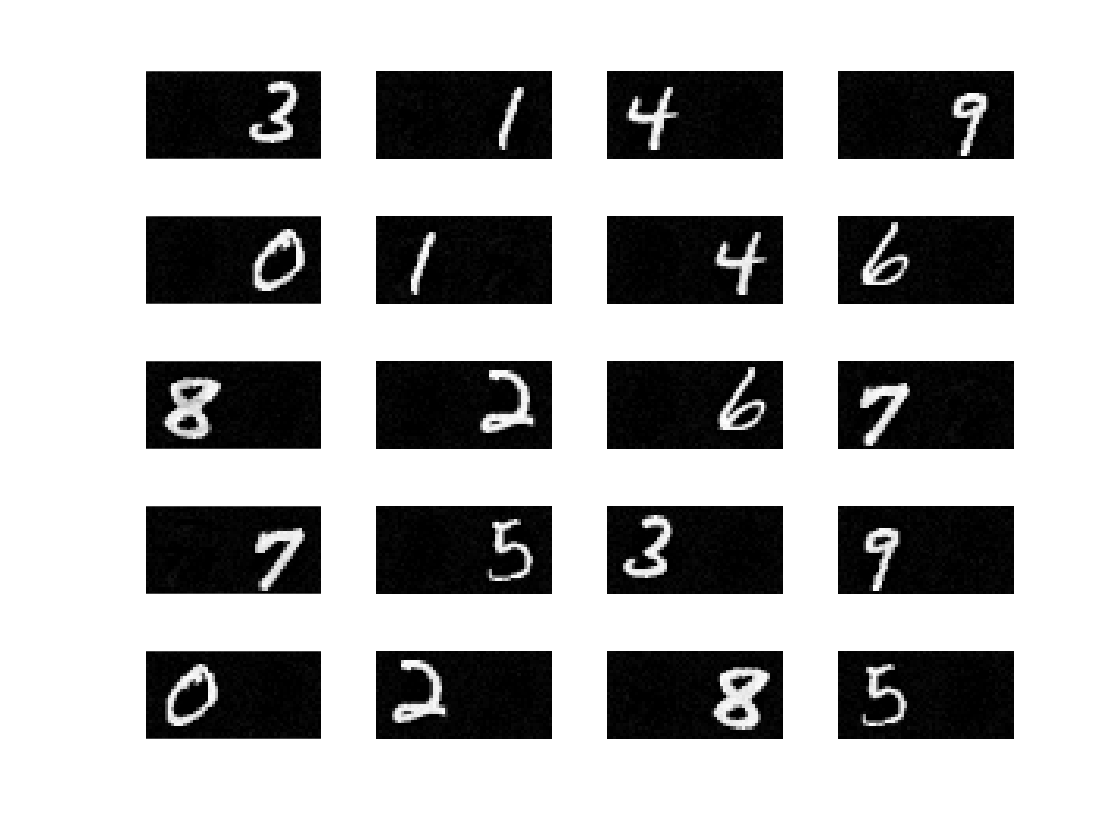
\includegraphics[width=\linewidth]{odl_best_basis_better}
\endminipage\hfill
\minipage{0.25\textwidth}%
  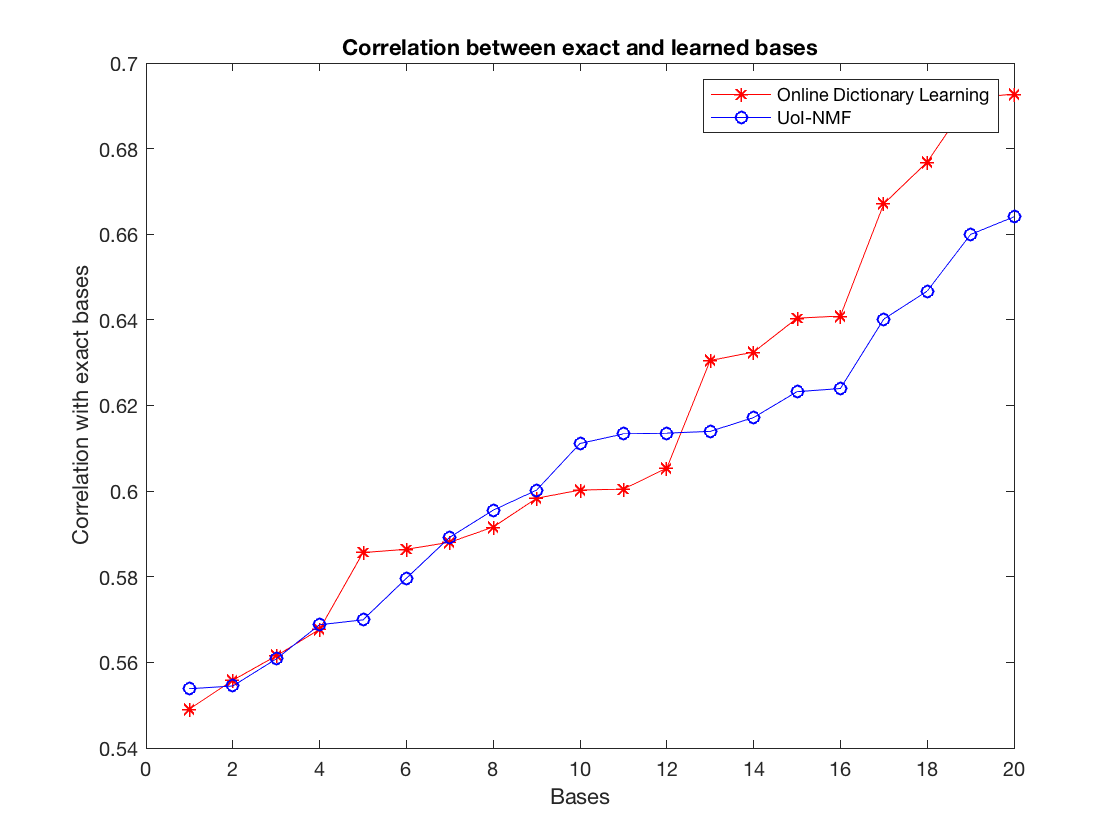
\includegraphics[width=\linewidth]{corr_2in1}
\endminipage
\minipage{0.25\textwidth}%
  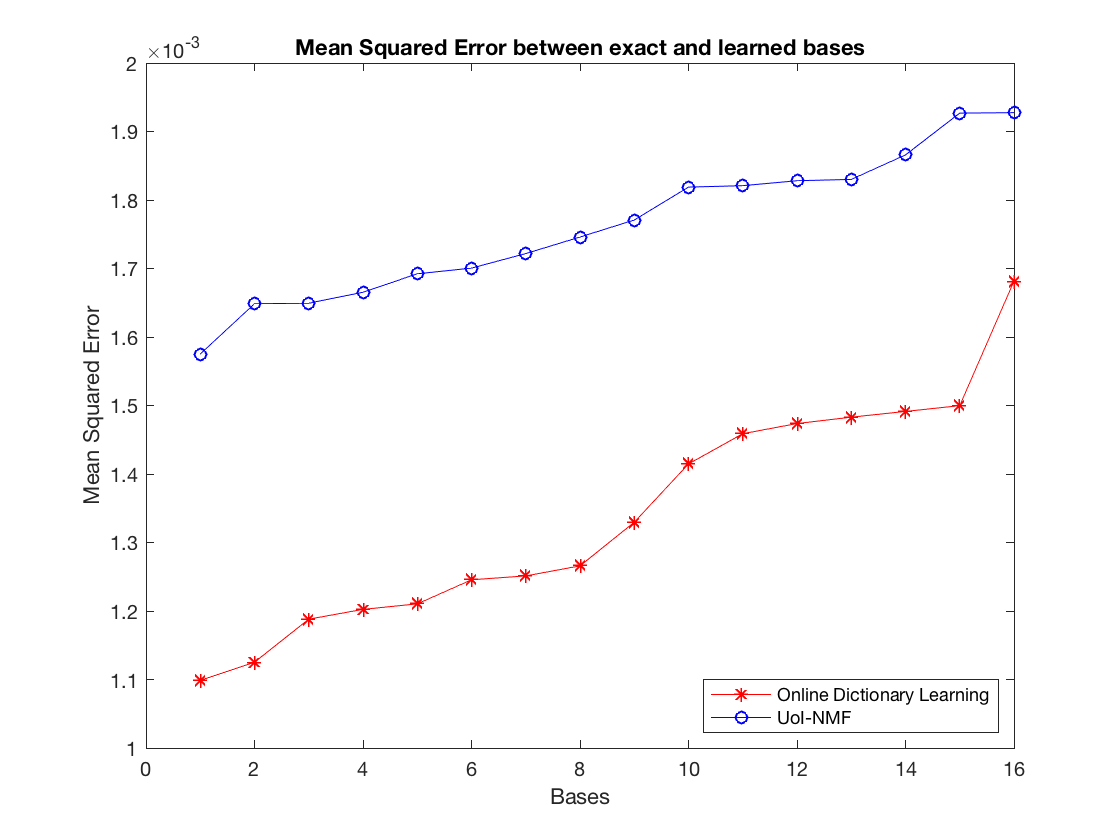
\includegraphics[width=\linewidth]{mse_2in1}
\endminipage
\caption{First $5\times 4$ images: 20 bases learned by \textit{UoI-NMF\textsubscript{cluster}} for the high noise MNIST two digits data. Second $5\times 4$ images: 20 bases learned by \textit{Online Dictionary Learning} for the same dataset. Third figure: Correlation between exact and learned bases for \textit{UoI-NMF\textsubscript{cluster}} and \textit{Online Dictionary Learning}. Fourth figure: Mean Squared Error between exact and learned bases for \textit{UoI-NMF\textsubscript{cluster}} and \textit{Online Dictionary Learning}. }\label{fig:mnist_4}
\end{figure*}

%-Swimmer-%
\begin{figure*}[!htb]
\centering
\minipage{0.25\textwidth}
  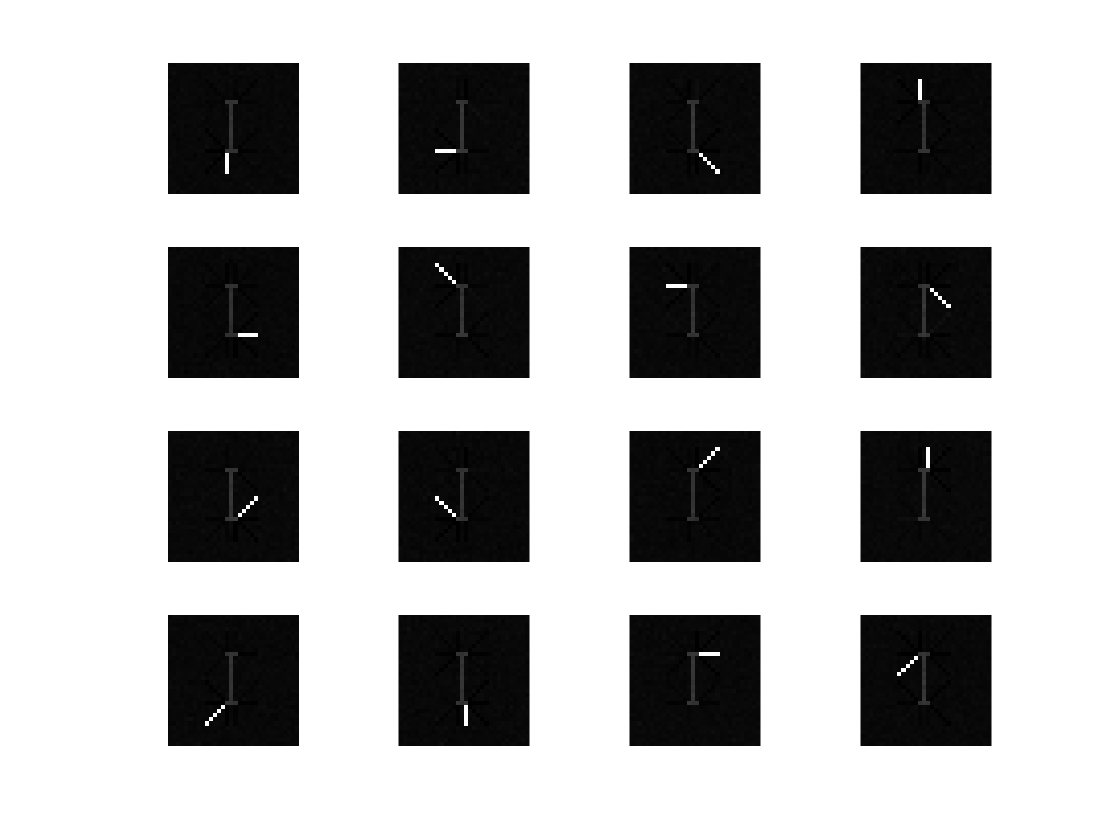
\includegraphics[width=\linewidth]{swimmer_uoi_best_basis}
\endminipage\hfill
\minipage{0.25\textwidth}
  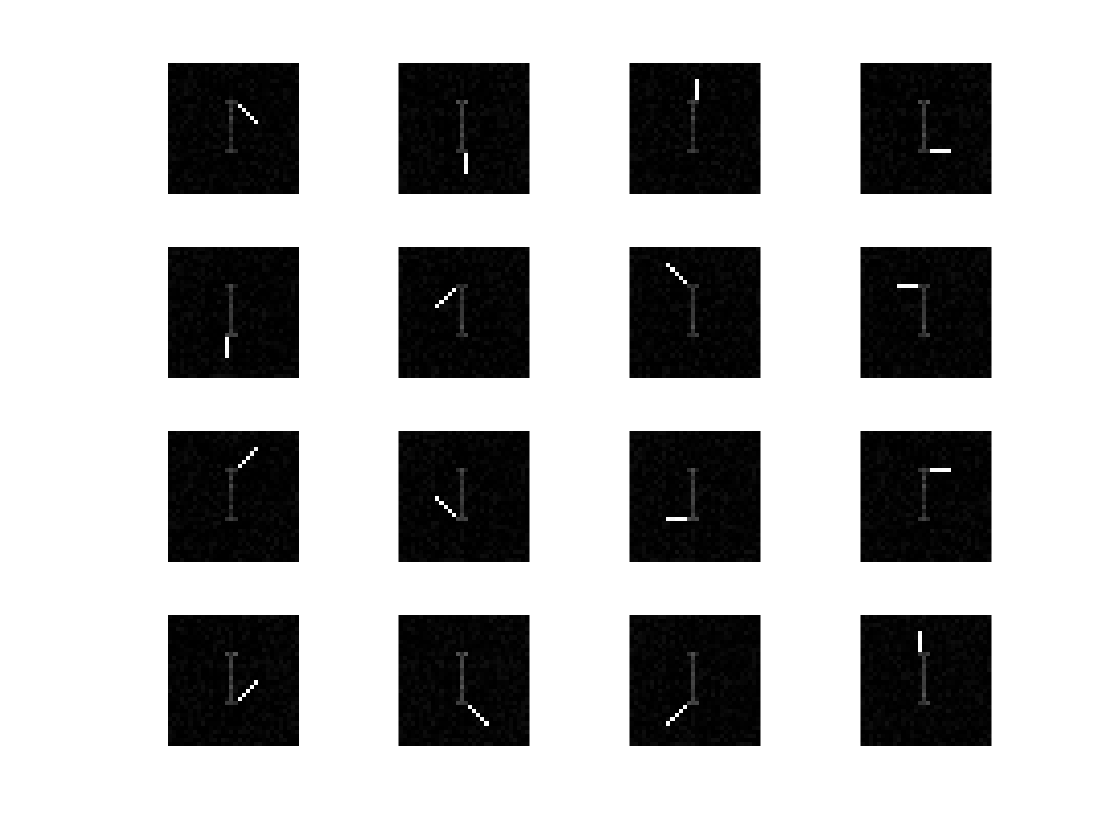
\includegraphics[width=\linewidth]{swimmer_odl_best_641}
\endminipage\hfill
\minipage{0.25\textwidth}%
  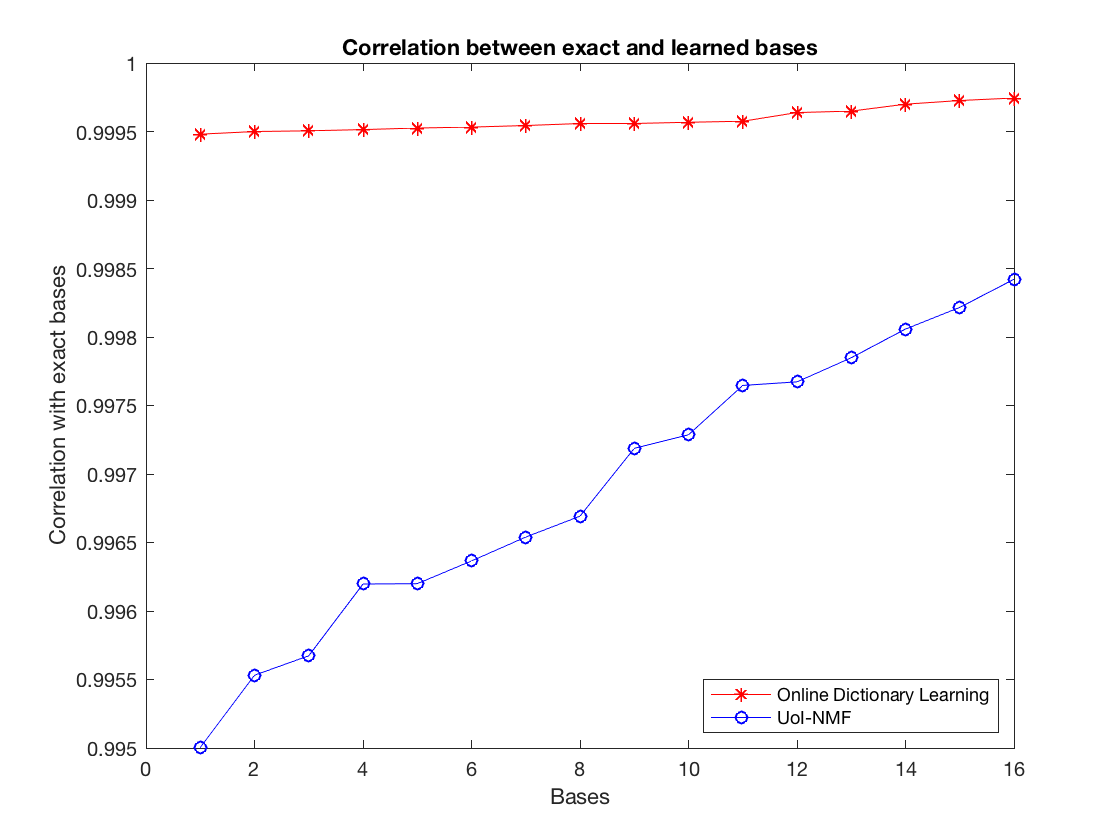
\includegraphics[width=\linewidth]{swimmer_corr_2in1}
\endminipage
\minipage{0.25\textwidth}%
  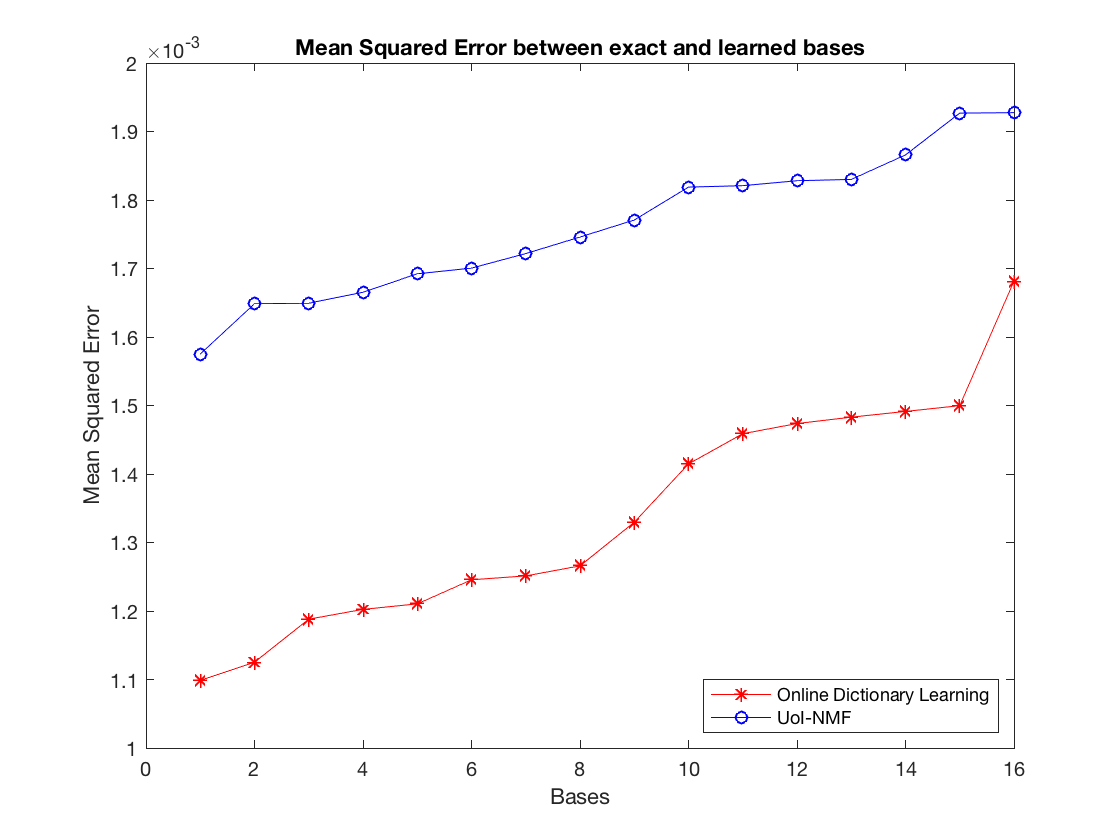
\includegraphics[width=\linewidth]{swimmer_mse_2in1}
\endminipage
\caption{First $4\times 4$ images: 16 bases learned by \textit{UoI-NMF\textsubscript{cluster}} for the
high noise Swimmer data. Second $4\times 4$ images: 16 bases learned by \textit{Online Dictionary Learning} for the same dataset. Third figure: Correlation between exact and learned bases for \textit{UoI-NMF\textsubscript{cluster}} and \textit{Online Dictionary Learning}. Fourth figure: Mean Squared Error between exact and learned bases for \textit{UoI-NMF\textsubscript{cluster}} and \textit{Online Dictionary Learning}. }\label{fig:swimmer_4}
\end{figure*}

%-%-%-%-%-%-%-%-%-%-%-%-%-%-%-%-%-%-%-%-%-%-%-%-%-%-%-%-%-%-%-%-%-%-%-%
After 1,000 iterations, the performance metrics as well as the learned atoms are shown in Fig. 1 for MNIST 2-digits dataset, side by side with \textit{UoI-NMF\textsubscript{cluster}}. The corresponding results for Swimmer dataset are shown in Fig. 2.

We can tell from the metrics that \textit{Online Dictionary Learning} has a slightly better accuracy than \textit{UoI-NMF\textsubscript{cluster}}. Both methods learned the bases/parts pretty well. Moreover, since \textit{Online Dictionary Learning} does not have the clustering part as in \textit{UoI-NMF\textsubscript{cluster}}, it runs faster, as is shown in Table. I.

\begin{table}[htbp]
\caption{Time Cost of the Two Methods}
\begin{center}
\begin{tabular}{|c|c|c|}
\hline
\textbf{Dataset}&\multicolumn{2}{|c|}{\textbf{Time Cost (sec)}} \\
\cline{2-3}
 & \textbf{\textit{UoI-NMF\textsubscript{cluster}}}& \textbf{\textit{Online Dictionary Learning}} \\
\hline
MNIST 2-digits & 112.46 & 1.89 \\
\hline
Swimmer & 213.82 & 2.29 \\
\hline
\end{tabular}
\label{tab1}
\end{center}
\end{table}

A large amount of time used by \textit{UoI-NMF\textsubscript{cluster}} is spent on clustering to get strong signal on the bases, which means \textit{UoI-NMF\textsubscript{cluster}} is more robust. Table. II \& III endorse this conclusion by showing reconstruction errors of the two methods with noisy and original data. We can see that both methods have similar reconstruction errors on noisy data. But \textit{UoI-NMF\textsubscript{cluster}} has a much lower reconstruction error on original data. We consider it as a benefit of the stronger bases learned by \textit{UoI-NMF\textsubscript{cluster}}. We also observed that in multiple runs, \textit{UoI-NMF\textsubscript{cluster}} inclines to give stable results of good quality whereas \textit{Online Dictionary Learning} could occasionally get polluted by the noise and get poor results.

\begin{table}[htbp]
\caption{Reconstruction Error with Noisy Data}
\begin{center}
\begin{tabular}{|c|c|c|}
\hline
\textbf{Dataset}&\multicolumn{2}{|c|}{\textbf{Reconstruction Error}} \\
\cline{2-3}
 & \textbf{\textit{UoI-NMF\textsubscript{cluster}}}& \textbf{\textit{Online Dictionary Learning}} \\
\hline
MNIST 2-digits & 192.9003 & 195.2450 \\
\hline
Swimmer & 242.0457 & 274.0686 \\
\hline
\end{tabular}
\label{tab2}
\end{center}
\end{table}

\begin{table}[htbp]
\caption{Reconstruction Error with Original Data}
\begin{center}
\begin{tabular}{|c|c|c|}
\hline
\textbf{Dataset}&\multicolumn{2}{|c|}{\textbf{Reconstruction Error}} \\
\cline{2-3}
 & \textbf{\textit{UoI-NMF\textsubscript{cluster}}}& \textbf{\textit{Online Dictionary Learning}} \\
\hline
MNIST 2-digits & 44.7821 & 238.2057 \\
\hline
Swimmer & 57.4769 & 261.9353 \\
\hline
\end{tabular}
\label{tab3}
\end{center}
\end{table}

\section{CONCLUSION}

We proposed a new application of \textit{Online Dictionary Learning} to the task of parts-based decomposition of noisy data in two datasets and compared the performance with the state-of-the-art method \textit{UoI-NMF\textsubscript{cluster}}. We found that both methods could find the actual bases in the process of dimension reduction for noisy data. \textit{UoI-NMF\textsubscript{cluster}} takes longer time, mainly due to the DBSCAN clustering step. However, we found this step crucial for the robustness. The clustering step indeed consolidated the learned bases so that they are more robust to noise. \textit{Online Dictionary Learning}, on the other hand, runs faster and has the potential of dealing with large amount of data, in an online or streaming way. In [When Does Non-Negative Matrix Factorization
Give a Correct Decomposition into Parts], it shows that both methods show the same mathematical foundation. That is why both could find the parts-based components.

\section{ACKNOWLEDGMENT}

The author would like to thank Shashanka Ubaru for providing thought-provoking ideas about sparse coding, dictionary learning and non-convex optimization.

The IEEEtran class file is used to format your paper and style the text. All margins,
column widths, line spaces, and text fonts are prescribed; please do not
alter them. You may note peculiarities. For example, the head margin
measures proportionately more than is customary. This measurement
and others are deliberate, using specifications that anticipate your paper
as one part of the entire proceedings, and not as an independent document.
Please do not revise any of the current designations.

%-%-%-%-%-%-%-%-%-%-%-%-%-%-%-%-%-%-%-%-%-%-%-%-%-%-%-%-%-%-%-%-%-%-%-%
\section{Prepare Your Paper Before Styling}
Before you begin to format your paper, first write and save the content as a
separate text file. Complete all content and organizational editing before
formatting. Please note sections \ref{AA}--\ref{SCM} below for more information on
proofreading, spelling and grammar.

Keep your text and graphic files separate until after the text has been
formatted and styled. Do not number text heads---{\LaTeX} will do that
for you.

\subsection{Abbreviations and Acronyms}\label{AA}
Define abbreviations and acronyms the first time they are used in the text,
even after they have been defined in the abstract. Abbreviations such as
IEEE, SI, MKS, CGS, ac, dc, and rms do not have to be defined. Do not use
abbreviations in the title or heads unless they are unavoidable.

\subsection{Units}
\begin{itemize}
\item Use either SI (MKS) or CGS as primary units. (SI units are encouraged.) English units may be used as secondary units (in parentheses). An exception would be the use of English units as identifiers in trade, such as ``3.5-inch disk drive''.
\item Avoid combining SI and CGS units, such as current in amperes and magnetic field in oersteds. This often leads to confusion because equations do not balance dimensionally. If you must use mixed units, clearly state the units for each quantity that you use in an equation.
\item Do not mix complete spellings and abbreviations of units: ``Wb/m\textsuperscript{2}'' or ``webers per square meter'', not ``webers/m\textsuperscript{2}''. Spell out units when they appear in text: ``. . . a few henries'', not ``. . . a few H''.
\item Use a zero before decimal points: ``0.25'', not ``.25''. Use ``cm\textsuperscript{3}'', not ``cc''.)
\end{itemize}

\subsection{Equations}
Number equations consecutively. To make your
equations more compact, you may use the solidus (~/~), the exp function, or
appropriate exponents. Italicize Roman symbols for quantities and variables,
but not Greek symbols. Use a long dash rather than a hyphen for a minus
sign. Punctuate equations with commas or periods when they are part of a
sentence, as in:
\begin{equation}
a+b=\gamma\label{eq}
\end{equation}

Be sure that the
symbols in your equation have been defined before or immediately following
the equation. Use ``\eqref{eq}'', not ``Eq.~\eqref{eq}'' or ``equation \eqref{eq}'', except at
the beginning of a sentence: ``Equation \eqref{eq} is . . .''

\subsection{\LaTeX-Specific Advice}

Please use ``soft'' (e.g., \verb|\eqref{Eq}|) cross references instead
of ``hard'' references (e.g., \verb|(1)|). That will make it possible
to combine sections, add equations, or change the order of figures or
citations without having to go through the file line by line.

Please don't use the \verb|{eqnarray}| equation environment. Use
\verb|{align}| or \verb|{IEEEeqnarray}| instead. The \verb|{eqnarray}|
environment leaves unsightly spaces around relation symbols.

Please note that the \verb|{subequations}| environment in {\LaTeX}
will increment the main equation counter even when there are no
equation numbers displayed. If you forget that, you might write an
article in which the equation numbers skip from (17) to (20), causing
the copy editors to wonder if you've discovered a new method of
counting.

{\BibTeX} does not work by magic. It doesn't get the bibliographic
data from thin air but from .bib files. If you use {\BibTeX} to produce a
bibliography you must send the .bib files.

{\LaTeX} can't read your mind. If you assign the same label to a
subsubsection and a table, you might find that Table I has been cross
referenced as Table IV-B3.

{\LaTeX} does not have precognitive abilities. If you put a
\verb|\label| command before the command that updates the counter it's
supposed to be using, the label will pick up the last counter to be
cross referenced instead. In particular, a \verb|\label| command
should not go before the caption of a figure or a table.

Do not use \verb|\nonumber| inside the \verb|{array}| environment. It
will not stop equation numbers inside \verb|{array}| (there won't be
any anyway) and it might stop a wanted equation number in the
surrounding equation.

\subsection{Some Common Mistakes}\label{SCM}
\begin{itemize}
\item The word ``data'' is plural, not singular.
\item The subscript for the permeability of vacuum $\mu_{0}$, and other common scientific constants, is zero with subscript formatting, not a lowercase letter ``o''.
\item In American English, commas, semicolons, periods, question and exclamation marks are located within quotation marks only when a complete thought or name is cited, such as a title or full quotation. When quotation marks are used, instead of a bold or italic typeface, to highlight a word or phrase, punctuation should appear outside of the quotation marks. A parenthetical phrase or statement at the end of a sentence is punctuated outside of the closing parenthesis (like this). (A parenthetical sentence is punctuated within the parentheses.)
\item A graph within a graph is an ``inset'', not an ``insert''. The word alternatively is preferred to the word ``alternately'' (unless you really mean something that alternates).
\item Do not use the word ``essentially'' to mean ``approximately'' or ``effectively''.
\item In your paper title, if the words ``that uses'' can accurately replace the word ``using'', capitalize the ``u''; if not, keep using lower-cased.
\item Be aware of the different meanings of the homophones ``affect'' and ``effect'', ``complement'' and ``compliment'', ``discreet'' and ``discrete'', ``principal'' and ``principle''.
\item Do not confuse ``imply'' and ``infer''.
\item The prefix ``non'' is not a word; it should be joined to the word it modifies, usually without a hyphen.
\item There is no period after the ``et'' in the Latin abbreviation ``et al.''.
\item The abbreviation ``i.e.'' means ``that is'', and the abbreviation ``e.g.'' means ``for example''.
\end{itemize}
An excellent style manual for science writers is \cite{b7}.

\subsection{Authors and Affiliations}
\textbf{The class file is designed for, but not limited to, six authors.} A
minimum of one author is required for all conference articles. Author names
should be listed starting from left to right and then moving down to the
next line. This is the author sequence that will be used in future citations
and by indexing services. Names should not be listed in columns nor group by
affiliation. Please keep your affiliations as succinct as possible (for
example, do not differentiate among departments of the same organization).

\subsection{Identify the Headings}
Headings, or heads, are organizational devices that guide the reader through
your paper. There are two types: component heads and text heads.

Component heads identify the different components of your paper and are not
topically subordinate to each other. Examples include Acknowledgments and
References and, for these, the correct style to use is ``Heading 5''. Use
``figure caption'' for your Figure captions, and ``table head'' for your
table title. Run-in heads, such as ``Abstract'', will require you to apply a
style (in this case, italic) in addition to the style provided by the drop
down menu to differentiate the head from the text.

Text heads organize the topics on a relational, hierarchical basis. For
example, the paper title is the primary text head because all subsequent
material relates and elaborates on this one topic. If there are two or more
sub-topics, the next level head (uppercase Roman numerals) should be used
and, conversely, if there are not at least two sub-topics, then no subheads
should be introduced.

\subsection{Figures and Tables}
\paragraph{Positioning Figures and Tables} Place figures and tables at the top and
bottom of columns. Avoid placing them in the middle of columns. Large
figures and tables may span across both columns. Figure captions should be
below the figures; table heads should appear above the tables. Insert
figures and tables after they are cited in the text. Use the abbreviation
``Fig.~\ref{fig}'', even at the beginning of a sentence.

\begin{table}[htbp]
\caption{Table Type Styles}
\begin{center}
\begin{tabular}{|c|c|c|c|}
\hline
\textbf{Table}&\multicolumn{3}{|c|}{\textbf{Table Column Head}} \\
\cline{2-4}
\textbf{Head} & \textbf{\textit{Table column subhead}}& \textbf{\textit{Subhead}}& \textbf{\textit{Subhead}} \\
\hline
copy& More table copy$^{\mathrm{a}}$& &  \\
\hline
\multicolumn{4}{l}{$^{\mathrm{a}}$Sample of a Table footnote.}
\end{tabular}
\label{tab1}
\end{center}
\end{table}

\begin{figure}[htbp]
\centerline{\includegraphics[width=4cm]{fig1.png}}
\caption{Example of a figure caption.}
\label{fig}
\end{figure}

Figure Labels: Use 8 point Times New Roman for Figure labels. Use words
rather than symbols or abbreviations when writing Figure axis labels to
avoid confusing the reader. As an example, write the quantity
``Magnetization'', or ``Magnetization, M'', not just ``M''. If including
units in the label, present them within parentheses. Do not label axes only
with units. In the example, write ``Magnetization (A/m)'' or ``Magnetization
\{A[m(1)]\}'', not just ``A/m''. Do not label axes with a ratio of
quantities and units. For example, write ``Temperature (K)'', not
``Temperature/K''.

\section*{Acknowledgment}

The preferred spelling of the word ``acknowledgment'' in America is without
an ``e'' after the ``g''. Avoid the stilted expression ``one of us (R. B.
G.) thanks $\ldots$''. Instead, try ``R. B. G. thanks$\ldots$''. Put sponsor
acknowledgments in the unnumbered footnote on the first page.

\section*{References}

Please number citations consecutively within brackets \cite{b1}. The
sentence punctuation follows the bracket \cite{b2}. Refer simply to the reference
number, as in \cite{b3}---do not use ``Ref. \cite{b3}'' or ``reference \cite{b3}'' except at
the beginning of a sentence: ``Reference \cite{b3} was the first $\ldots$''

Number footnotes separately in superscripts. Place the actual footnote at
the bottom of the column in which it was cited. Do not put footnotes in the
abstract or reference list. Use letters for table footnotes.

Unless there are six authors or more give all authors' names; do not use
``et al.''. Papers that have not been published, even if they have been
submitted for publication, should be cited as ``unpublished'' \cite{b4}. Papers
that have been accepted for publication should be cited as ``in press'' \cite{b5}.
Capitalize only the first word in a paper title, except for proper nouns and
element symbols.

For papers published in translation journals, please give the English
citation first, followed by the original foreign-language citation \cite{b6}.

\begin{thebibliography}{00}

\bibitem{b1} Mallat, S, ``A wavelet tour of signal processing'' 2nd ed., Academic Press, New York 1999.

\bibitem{b2} J. Clerk Maxwell, A Treatise on Electricity and Magnetism, 3rd ed., vol. 2. Oxford: Clarendon, 1892, pp.68--73.

\bibitem{b3} I. S. Jacobs and C. P. Bean, ``Fine particles, thin films and exchange anisotropy,'' in Magnetism, vol. III, G. T. Rado and H. Suhl, Eds. New York: Academic, 1963, pp. 271--350.

\bibitem{b4} K. Elissa, ``Title of paper if known,'' unpublished.

\bibitem{b5} R. Nicole, ``Title of paper with only first word capitalized,'' J. Name Stand. Abbrev., in press.

\bibitem{b6} Y. Yorozu, M. Hirano, K. Oka, and Y. Tagawa, ``Electron spectroscopy studies on magneto-optical media and plastic substrate interface,'' IEEE Transl. J. Magn. Japan, vol. 2, pp. 740--741, August 1987 [Digests 9th Annual Conf. Magnetics Japan, p. 301, 1982].

\bibitem{b7} M. Young, The Technical Writer's Handbook. Mill Valley, CA: University Science, 1989.

\bibitem{b8} Donoho D, Stodden V. When does non-negative matrix factorization give a correct decomposition into parts?. InAdvances in neural information processing systems 2004 (pp. 1141-1148).

\end{thebibliography}
\vspace{12pt}


\end{document}
